\chapter{Proposed Algorithm}\label{kap4}

The main goal of this thesis is to propose an algorithm to repair an XML document violating functional dependencies defined for this document. We use an XML tree and tree tuples to represent XML data. We would like our algorithm to have the following features::

\begin{itemize}
	\item Incorporation of a weight model into the XML data representation to provide the selection of repair candidates with the lowest modification cost.
    \item Involvement of a user in the process of finding and applying repair candidates.
    \item Application of a single repair candidate at the time and then recalculate repair candidates again to prevent using unnecessary repairs to repair one violation and also to prevent of introducing new violations, which will not be repaired.
    \item The paths which form a functional dependency are described with XPath language \cite{xpath}, where only paths with basic construction are allowed (only path constructed with "/", "//" or "@", no wildcards, "[]" or another constructs are allowed).
    \item We introduce a new concept of the so-called repair group, which clusters repair candidates (repairs for repairing one FD violation) repairing the same violation, or modifying the same part of the XML tree.
\end{itemize}


\section{Repairing Algorithm}

The proposed algorithm is based on the algorithm described in \ref{RepConstAnswers} presented in \cite{RepAndConsistentAnswer}. This algorithm was chosen because of simple representation of the XML data using a concept which corresponds with concept used in relational databases. Another reason, besides modification of node value as an update operation, is using also marking particular node information as unreliable, which can reveal forgotten inconsistencies in the data.

\begin{algorithm}
\caption{Repair RW-XML tree}
\label{propAlgo}
\begin{algorithmic}[1]
\REQUIRE{\ \\
$RXT = \langle RT, \omega \rangle$: RW-XML tree conforming to DTD $D$\\
$\mathcal{FD} = {F_1, \dots, F_m}$: Set of functional dependencies}
\ENSURE a unique repaired RW-XML tree

\STATE $resultRXT = RXT$
\WHILE{$resultRXT \not \models_w \mathcal{FD}$}
    \STATE $S = \emptyset$ \COMMENT Set of repair groups
    \FORALL{$(F: S \rightarrow p) \in \mathcal{FD}$ s.t. $RXT \not \models_w F$}
    	\FORALL{$t_1, t_2$ tuples of $RXT$ s.t. $t_1, t_2$ do not weakly satisfy $F$}
		    \STATE $S = S \cup computeRepairGroup(F, t_1, t_2, RXT, S)$
	    \ENDFOR
    \ENDFOR

    \STATE $R = getRepair(S, RXT)$
    \STATE $resultRXT = applyRepair(R, resultRXT)$
\ENDWHILE

\end{algorithmic}
\end{algorithm}

The algorithm is split into three steps, where the second and the third step are repeated until all violations are repaired. In the first step, XML document and FDs are loaded, and XML tree with corresponding tree tuples are created. Next step of the algorithm computes repair groups containing repair candidates for FD violations. In the third step the chosen repair candidate is applied to an XML tree. In Algorithm \ref{propAlgo} we can see the simplified process of repairing XML FD violations, which covers the second and the third step of the whole algorithm.

\subsection{Initial data model}

To represent an XML document we use an extended R-XML tree (Definition \ref{rxmlTree}), called RW-XML tree, which has weights assigned to each node of the tree. The weight of a node is from interval $[0,1]$ and indicates correctness of the data the particular node holds, meaning the higher the weight is, the more correct that particular node is. The weights are used to measure the cost of repair candidates, where candidate with the lowest cost is picked to be applied to the XML tree. This is also the first place where some kind of user interaction can be implemented. The user could assign the weights to nodes manually or could use some sort of statistical methods to generate them automatically. If the user does not assign weights nor does he use statistical methods, a default weight is assigned to all nodes.

\begin{example}
Consider the XML document and corresponding XML tree from Example \ref{example1}. Let us assign weights to nodes defined by XPath constructs shown in Table \ref{weightTab}. The XML tree with assigned custom and also default weights is shown in Fig. \ref{weightsFig}.

\begin{table}[h]
\begin{tabular}{r | c}
XPath & weight\\\hline
$/bib/book/title/text()$ & 0.8\\
$/bib/book/written\_by/author$ & 0.6\\
$/bib/book/written\_by/author/@ano$ & 0.1\\
\end{tabular}
\caption{Table of custom weights assigned to the XML tree.}
\label{weightTab}
\end{table}

\begin{figure}[H]
    \centering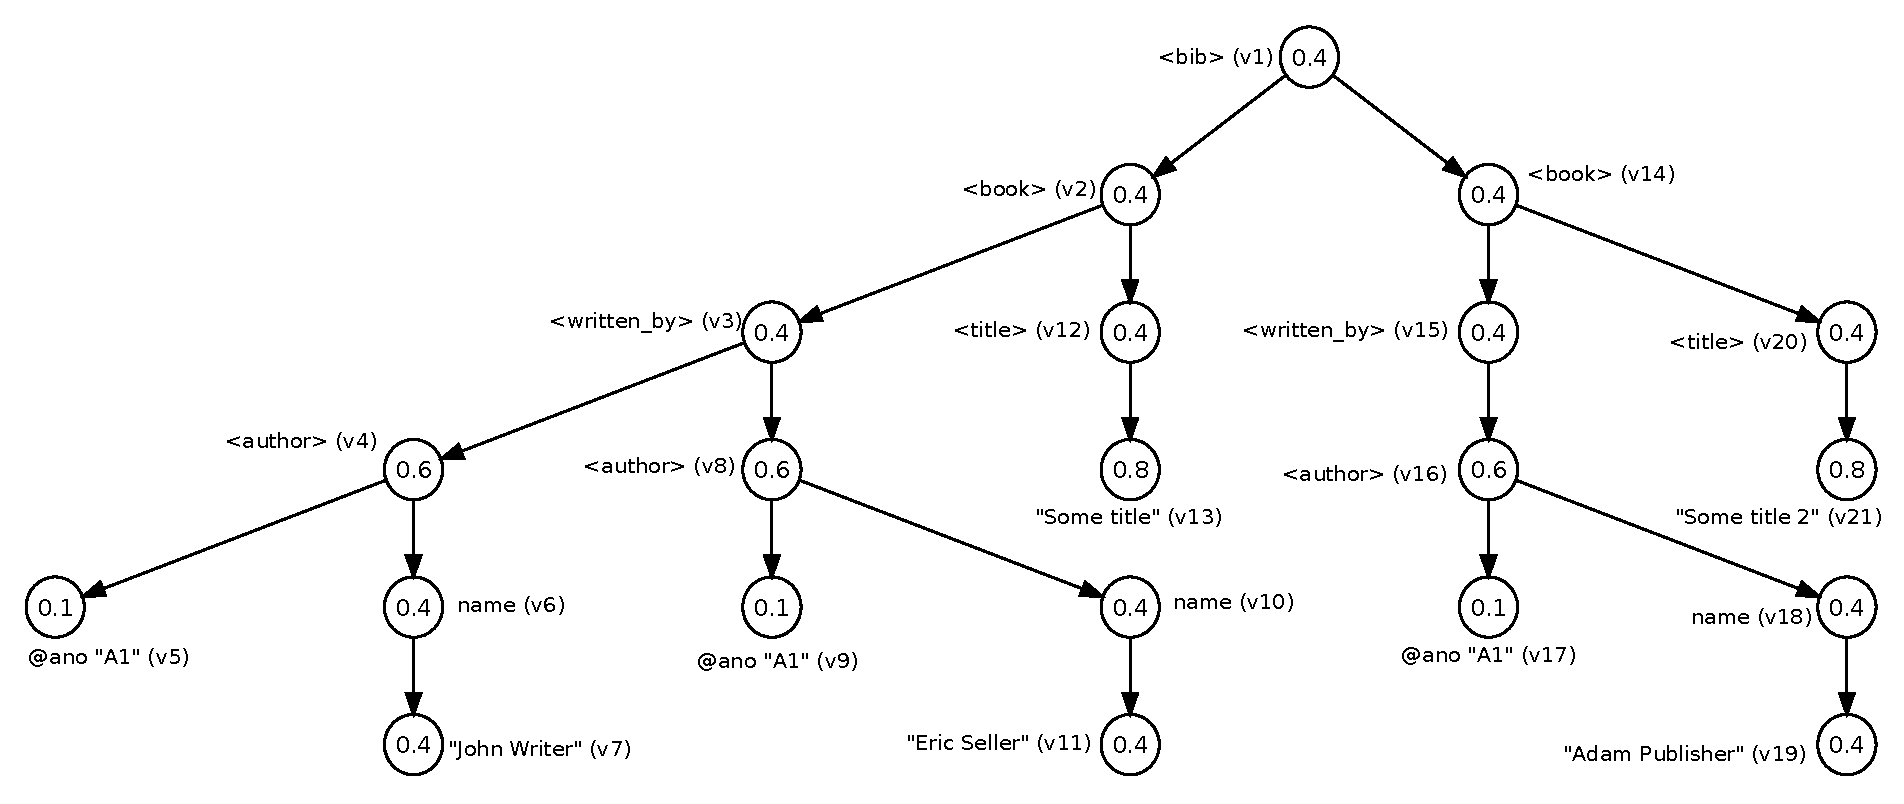
\includegraphics[width=\textwidth]{weights}
	\caption{The XML tree with assigned weights to the nodes.} \label{weightsFig}
\end{figure}
\qed
\end{example}


\begin{define}[RW-XML tree]
A {\sl RW-XML tree} is a pair $RWXT = \langle RXT, \omega \rangle$, where $RXT$ is an R-XML tree and $\omega$ is a weight function from $N_T$ to $[0,1]$.\qed
\end{define}

After creating the RW-XML tree from input XML data, a set of tree tuples (defined in Definition \ref{treeTuple}) is constructed. Since the set $paths(D)$, containing all possible paths defined in DTD $D$, can be infinite (DTD can define recursive structure of elements), the actual content of $paths(D)$ is modified to reflect the current structure of the RW-XML tree. Since definition of a tree tuple says that answer to the path $p$ contains at most one element, our modification of $paths(D)$ has no effect on constructing tree tuples if a DTD defines some optional path which is not defined for the RW-XML tree $RWXT$ (the set $p(RWXT)$ is empty).

Functional dependencies as defined in Definition \ref{fd1} consist of paths described with XPath. As was described before, these paths can only have basic structure shown in Example \ref{pathsExample}.

\begin{example}\label{pathsExample}
Example of paths that can be used in functional dependencies:
\begin{verbatim}
//bib/book/author
/bib/book/author/@ano
/bib/book/author/name/text()
\end{verbatim}
\end{example}

\subsection{Computing Repair Groups}

With RW-XML tree $RWXT$ and corresponding tree tuples from input data created, we can now proceed to compute repair groups. Repair group is a set of repair candidates, which repairs the same FD or modifies the same part of $RWXT$. Each repair candidate is a pair of functions $\delta$ and $\varrho$ ($\langle \delta, \varrho \rangle$), which either modifies value of an RW-XML tree node ($\delta$ is defined) or marks a node as unreliable ($\varrho$ is defined). The $\delta$ function of a repair candidate is defined the same way as in the XML tree (Definition \ref{xmlTree}) and defines a new value of the RW-XML tree node. Similarly, the $\varrho$ function defines the node which is marked as unreliable.

To be able to compute repair groups, we need to decide which FDs violate $RWXT$. This can be achieved by finding all tree tuple pairs that do not weakly satisfy particular FD (Definition \ref{weakSatisf}). A repair group is then computed for each tuple pair (line 6 in Algorithm \ref{propAlgo}).

The function \texttt{computeRepairGroup()} responsible for creating the repair group is shown in Algorithm \ref{repairGroupAlgo}. The function gets an RW-XML tree, a functional dependency $F$, tuples $t_1$, $t_2$ and a set of repair groups $RGS$ and computes the repair group containing repair candidates as follows:

\begin{enumerate}
	\item First the repair candidates are created using function \texttt{computeRepairs()} from Algorithm \ref{repAlgo} (line 1). Since an R-XML tree is a special case of RW-XML tree where all the weights are equal to zero, we can pass RW-XML tree as a parameter to this function.
    \item Next a check is performed whether the repair candidates intersect other candidates from existing repair groups (line 2)
    \begin{itemize}
    	\item If the candidates intersect with some group, they are added to this group (line 3)
        \item Otherwise a new repair group containing repair candidates is created (line 5)
    \end{itemize}
\end{enumerate}

\begin{algorithm}
\floatname{algorithm}{Function}
\caption{$computeRepairGroup(F, t_1, t_2, RXT, RGS)$}
\label{repairGroupAlgo}
\begin{algorithmic}[1]
\REQUIRE{\ \\
$RXT = \langle T, \omega \rangle$: RW-XML tree conforming to DTD $D$\\
$F: X \rightarrow p$ functional dependency\\
$t_1, t_2$ tuples of $RXT$\\
$RGS$ set of repair groups}
\ENSURE $RG$: repair group

\STATE $S = computeRepairs(F, t_1, t_2, RXT)$ \COMMENT set of repair candidates

\IF{$candidatesIntersectRepairGroups(S, RGS)$}
\STATE $RG = getIntersectingRepairGroup(S, RGS)$
\ELSE
\STATE $RG = createNewRepairGroup(S)$
\ENDIF

\RETURN $RG$
\end{algorithmic}
\end{algorithm}

Example \ref{repairExample} demostrates repair candidates of one repair group modifying node values and marking nodes as unreliable.

\begin{example}\label{repairExample}
Consider XML data and functional dependency from Example \ref{fdrepairExample}, where XML data is graphically represented as XML tree $XT$ in Fig \ref{example1}. The $XT$ violates FD $$\{/bib/book, /bib/book/written\_by/author/@ano\} \rightarrow /bib/book/written\_by/author$$ because two authors of the same book have the same value of attribute $@ano$. One repair group with these repair candidates is created:
\begin{itemize}
	\item $R_1 = \langle \{\delta(v5) = \perp\},\varrho_{\{\}}(v) \rangle$
    \item $R_2 = \langle \{\delta(v9) = \perp\},\varrho_{\{\}}(v) \rangle$
    \item $R_3 = \langle \{\},\varrho_{\{v4,v5,v6,v7\}}(v) \rangle$
    \item $R_4 = \langle \{\},\varrho_{\{v8,v9,v10,v11\}}(v) \rangle$
    \item $R_5 = \langle \{\},\varrho_{\{v2,v3,\dots,v13\}}(v) \rangle$
\end{itemize}

First two repair candidates modify the value of an attribute $@ano$ by assigning newly generated value ($\perp$). Next two repair candidates mark each \emph{author} node with its child nodes that have the same $@ano$ attribute respectively. The last candidate marks as unreliable a whole subtree with the \emph{book} node holding \emph{authors} with the same attribute as the root node.\qed
\end{example}

\subsubsection{Weight model of a Repair Group}

In this section, we introduce a weight model for a repair group, which will be used in the next step of our repair algorithm. Before we define a weight of a repair group, let us introduce some important notations.

Being given a repair candidate $R$, $Modified_\delta(R)$ denotes the set of nodes modified by $\delta$ function from $R$. Analogously, we denote $Modified_\varrho(R)$ the set of nodes modified by $\varrho$ function. The count of nodes modified by repair candidate $R$ is denoted with $\lambda(R)$. Last, we denote $PS(R)$ a set of paths defining all nodes modified by $R$ (example of the set $PS(R)$ is shown in Example \ref{PSExample}).

\begin{example}\label{PSExample}
Consider the XML tree from Fig. \ref{example1} and a repair candidate, which marks nodes $v12$ and $v13$ as unreliable. Then the set $PS(R)$ contains the following paths:
\begin{verbatim}
/bib/book/title
/bib/book/title/text()
\end{verbatim}\qed
\end{example}


Since each repair candidate consists of a set of nodes which are modified (marked as unreliable or having a modified value), we can compute the cost of each candidate. It is important to say that unlike in original approach, we do not prefer repair candidates that modify the value of the nodes to those marking nodes as unreliable. Therefore we added a coefficient $k$ to the calculation of the repair candidate cost, so that the priority of repair candidate marking node as unreliable can be achieved. The definition of repair candidate cost is as follows:

\begin{define}[Repair Candidate Cost]
Being given an RW-XML tree $RXT$ and a repair candidate $R$, we define the {\sl cost} of $R$ as:
$$cost(R) = \sum_{u \in Modified_\delta(R)} \omega(u) + \sum_{v \in Modified_\varrho(R)} \omega(v) \cdot k,$$
where $k$ is the priority of repairing the candidate by modifying the node value in constrast to marking it unreliable.\qed
\end{define}

By default, $k$ is set to such value that the cost of repair candidate marking as an unreliable node will be higher than the one that modifies node value. However, this is another place where user can intervene and change the priority of repair candidates. We show in Example \ref{koefK} how $k$ can change the costs of repair candidates.

\begin{example}\label{koefK}
Consider XML tree $XT$ and repair candidates from Example \ref{repairExample}. The default weight of all nodes $v$ of $XT$ is $\omega(v) = 0.5$. If the coefficient $k = 1$, cost of repair candidates would be as follows: $cost(R_1) = 0.5$, $cost(R_2) = 0.5$, $cost(R_3) = 2$, $cost(R_4) = 2$ and $cost(R_5) = 6$.
Let us assume that a repair candidate with the lowest repair cost will be applied to $XT$. If we order costs of repair candidates from the lowest to the highest, we can see that candidates which have marked unreliable nodes are in the end (and will not be applied to $XT$).

However, if we set the coefficient $k = 0.1$, costs of candidates would be sorted as follows: $cost(R_3) = 0.2$, $cost(R_4) = 0.2$, $cost(R_1) = 0.5$, $cost(R_2)  = 0.5$ and $cost(R_5) = 0.6$. We can see that order of costs has significantly changed and the candidate which will be applied is $R_3$ (marking nodes as unreliable).\qed
\end{example}

And, finally, since a repair group is a set of repair candidates, its weight can be defined as follows:

\begin{define}[Repair Group weight]
Being given an RW-XML tree $RXT$ and a repair group $RG$, we define the {\sl weight} of $RG$ as the sum of costs of all repair candidates in the $RG$.
\end{define}

\subsection{Repair Candidate Selection and Application}

The last step of our algorithm can be divided into two parts, namely selection of the repair candidate and the subsequent application of the candidate to RW-XML tree.

\subsubsection{Selection of the Repair Candidate}

The previous step of the algorithm computes repair groups containing repair candidates, which can repair violations of provided FDs. From these candidates, we must choose the one that is applied to the RW-XML tree. Since we introduced a weight model to the repair group, we can use the weight of repair groups and the cost of repair candidates to choose a suitable candidate. In our approach, we introduce two distinct algorithms: first that does not involve the user in the process of selection and the second one that uses the user interaction.

The former algorithm simply selects the first repair group with the lowest weight, and from it the repair candidate with the lowest cost is selected.

The latter algorithm allows the user to choose the repair candidate which is the most suitable for his needs. Very important aspect of all user interactions in this kind of algorithm is that the user will not be willing to select more than, e.g., ten repairs. We could simply allow user to switch to the first selection algorithm, but that does not take in account previous user selections of repair candidates. Therefore, we introduce in this algorithm a functionality able to guess his next selection from selection done by the user before.

The function \texttt{selectRepairByUser()} responsible for selection of repair candidate involving user interactivity is shown in Algorithm \ref{selectUser}.

First it decides, whether the algorithm is in a state where the user is selecting repair candidates (the user selection mode), or the user leaves decision making on the algorithm using his previous selections (the guess mode) (line 2). If we are still in user selection mode, the user chooses from repair groups sorted by the weight the most convenient one, and from this group the user chooses the repair candidate that will be applied on RW-XML tree (line 3). Repair candidates in each repair group are also sorted by the cost, working as a hint for the user which repair would be chosen by the previous automatic method of selection. The last step of user selection mode is saving the information from selected repair candidate (line 4). This information consists of the FD which this candidate repairs, nodes the repair changes (their paths) and also whether the change was a value modification or marking a node as unreliable.

If the user has decided not to select repair candidates by himself anymore, the algorithm goes into the guess mode (starting at line 5). In this mode the algorithm checks all repair groups whether one of them contains a repair candidate that is sufficiently similar to some previously selected repair candidate (line 6-12). This similarity is checked by function \texttt{canBeUsedUserSelection()} shown in Algorithm \ref{canUserSel}. If neither of the candidates is sufficiently similar, the algorithm chooses the repair candidate with the lowest cost from the repair group with the lowest weight (line 13-14).

\begin{algorithm}[H]
\floatname{algorithm}{Function}
\caption{$selectRepairByUser(RGS, SR, t)$}
\label{selectUser}
\begin{algorithmic}[1]
\REQUIRE{\ \\
$RGS$ set of repair groups\\
$SR$: the set of repair candidates previously selected by the user\\
$t$: modified nodes count threshold of previously selected repair candidates\\}
\ENSURE $R$: repair candidate

\STATE $R = \emptyset$
\IF[the user selection mode]{$isUserSelection()$}
    \STATE $R = getRepairFromUser()$ \COMMENT{repair candidate selected by user}
    \STATE $saveSelectedRepair(SR, R)$
\ELSE[the guess mode]
    \FORALL{$RG$ in $RGS$}
        \FORALL[for all repair candidates in the repair group]{$RC$ in $RG$}
            \IF{$canBeUsedUserSelection(SR, t, RC)$}
                \RETURN $RC$
            \ENDIF
        \ENDFOR
    \ENDFOR
    \STATE $RG = getFirstRG(RGS)$ \COMMENT get the repair group with smallest weight
    \STATE $R = getFirstRepairCandidate(RG)$ \COMMENT get the repair candidate with the lowest cost
\ENDIF

\RETURN $R$
\end{algorithmic}
\end{algorithm}

The function \texttt{canBeUsedUserSelection()} gets the current repair candidate $RC$, the set of all previously selected repair candidates $SR$, and the modified nodes count threshold $t$ from interval $(0,1]$ of previously selected repair candidate and it determines whether the $RC$ is sufficiently similar to some repair candidate from $SR$. To be similar with some previously selected repair candidate $S$, $RC$ must repair the same $FD$ as $S$, it must use the same update operation as $S$ and $\lambda(RC) \geq \lceil\lambda(S) \cdot t\rceil$ (line 2). Furthermore, if $\lambda(RC) = \lceil\lambda(S) \cdot t\rceil$, the set of paths $PS(RC)$ must be a subset of $PS(S)$ (line 3). Otherwise, if $\lambda(RC) > \lceil\lambda(S) \cdot t\rceil$, there must exist a subset of $PS(S)$ with $\lceil\lambda(S) \cdot t\rceil$ elements that is a subset of $PS(RC)$. In other words, without taking into account the threshold $t$, if a repair candidate $R_1$ modifies some nodes, the sufficiently similar repair candidate $R_2$ is the one that modifies at least the same nodes as $R_1$ (when we say the same nodes we mean same paths representing those nodes). The threshold $t$ can reduce the number of modified nodes of some previously selected repair candidate $R_1$, which means that sufficiently similar repair candidate needs to modify fewer nodes that are similar with nodes modified by $R_1$. In Example \ref{tresholdExample} the usage of the threshold $t$ is shown.


\begin{algorithm}
\floatname{algorithm}{Function}
\caption{$canBeUsedUserSelection(SR, t, RC)$}
\label{canUserSel}
\begin{algorithmic}[1]
\REQUIRE{\ \\
$SR$: the set of previously selected repair candidates by the user\\
$t$: a suitability threshold $(0,1]$ of previously selected repair candidates\\
$RC$: the current repair candidate}
\ENSURE \TRUE\ if $RC$ is similar to some previous repair candidate.
\FORALL{$S$ in $SR$}
    \IF{$S$ repairs the same FD as $RC$ \AND $S$ use the same update operation as $RC$ \AND $\lceil\lambda(SC) \times t\rceil \leq \lambda(RC)$}
        \IF{$\lceil\lambda(SC) \times t\rceil = \lambda(RC)$ \AND $PS(RC) \subseteq PS(SC)$}
            \RETURN \TRUE
        \ENDIF
        \IF{$\lceil\lambda(SC) \times t\rceil < \lambda(RC)$ \AND there exists a subset $s$ of $PS(SC)$ with $\lceil\lambda(SC) \times t\rceil$ elements, that $s \subseteq$ $PS(RC)$}
            \RETURN \TRUE
        \ENDIF
   \ENDIF
\ENDFOR
\RETURN \FALSE
\end{algorithmic}
\end{algorithm}

\begin{example}\label{tresholdExample}
Consider repair candidate $R_1$ selected by user, that marks as unreliable two nodes and $PS(R_1) = \{/bib/book/title, /bib/book/title/text()\}$. Next, consider repair candidate $R_2$ with $PS(R_2) = \{/bib/book/title/text()\}$, that the modified node is marked as unreliable and both $R_1$ and $R_2$ repairs the same $FD$. If $t=1$, $R_2$ is not considered as sufficiently similar to $R_1$, because $\lceil\lambda(R_1) \times t\rceil > \lambda(R_2)$. However, if $t=0.5$, $\lceil\lambda(R_1) \times t\rceil = \lambda(R_2)$ and $PS(R_2) \subseteq PS(R_1)$, then $R_2$ is sufficiently similar to $R_1$.\qed
\end{example}

\subsubsection{Application of the Repair Candidate}

In this part, the selected repair candidate is finally applied to the RW-XML tree. If after this part the RW-XML tree does not violate any FDs, the whole repair algorithm ends at this point, otherwise repair groups are regenerated and the selection of the repair candidate part takes place again.

To apply the selected repair candidate $R$ to the RW-XML tree $RXT$ means to compose $\delta$ and $\varrho$ functions of $R$ with the corresponding functions of R-XML tree contained in $RXT$. These compositions are defined in Definition \ref{compDelta} and \ref{compVarrho}.

After application of the repair candidate, some of RW-XML tree nodes could become unreliable, which can lead to the situation that some of tree tuples are not anymore considered a tuple (it is no longer a maximal subtree). Therefore, before regeneration of repair groups we need to check all tree tuples to see whether they satisfy definition of tree tuple.
